\Chapter{Keresztfordítás}

\section{Formális nyelvek}

A formális nyelvek bevezetéséhez először is át kell tekintetni, az ábécé, a nyelv és nyelvtan fogalmát.

"Szimbólumok tetszőleges nemüres, véges halmazát ábécének nevezzük és V-vel jelöljük." (Dömösi Pál, Falucskai János, Horváth Géza, Mecsei Zoltán, Nagy Benedek - Formális Nyelvek és Automaták https://gyires.inf.unideb.hu/KMITT/b24/) Látható tehát, hogy az ábécét egy halmazként definiáljuk, mely nem üres halmaz és tetszőleges szimbólumokat tartalmaz. Bár az említett könyvben a definíció szerint V-vel jelölik az ábécét, általánosságban azt mondhatjuk, hogy nagybetűvel (A, B) esetleg $\Sigma$ karakterrel történik ennek jelölése.

"A V ábécé feletti szavak egy tetszőleges L halmazát a V ábécéből alkotott (formális) nyelvnek nevezzük" (Dömösi Pál, Falucskai János, Horváth Géza, Mecsei Zoltán, Nagy Benedek - Formális Nyelvek és Automaták https://gyires.inf.unideb.hu/KMITT/b24/), azaz a nyelv egy az adott ábécé felett értelmezett szavak tetszőleges halmaza lesz. Általánosan formális nyelveknek nevezünk minden olyan nyelvet, melyekben véges hosszúságú szavak generálhatók véges ábécékből. A programozási nyelvek alapvetően ilyen formális nyelvek.

Az informatikához kapcsolódóan az ilyen leírást a formális nyelvtannal jellemezzük, mely konkrétan egy formális nyelvet ír le.

A nyelvtan két nagy kategóriája a generatív és analitikus nyelvtan. Előbbi azt írja le, hogyan lehet előállítani az adott nyelvet egy adott szabályhalmazból, míg utóbbi az adott nyelv olvasását írja le, ugyancsak szabályokkal.
A generatív nyelvek tekintetében meg kell említeni azok osztályozását is. Ezt először az 1950-es években vetette fel Noam Chomsky nyelvész, mely osztályozást róla nevezték Chomsky-hierarchiának.

"Chomsky négy nyelvosztályt definiált. Ezeket számokkal jelölte, így van 0-ás, 1-es, 2-es és 3-as nyelvosztály. Az egyes nyelvosztályokban a helyettesítési szabályok alakjára vonatkozóan Chomsky az osztály sorszámának növekedésével egyre szigorúbb megkötéseket írt elő." (BACH IVÁN - Formális nyelvek https://www.typotex.hu/download/formalisnyelvek.pdf)

 Ez a besorolás 4 osztályba sorolja a nyelveket az alapján, hogy mennyire kifejezőek, illetve milyen szigorú megkötések vonatkoznak rájuk. Az alábbi táblázatban lehet összefoglalni az egyes csoportokat, azaz osztályok tulajdonságait.
 
\begin{table}
	\caption{Chomsky-hierarchia}
	\label{1. táblázat}
	\begin{tabular}{c|c|c|c|c}
		\textbf{Nyelvoszály} & \textbf{Nyelvtanok} & \textbf{Nyelvek} & \textbf{Automaták} & \textbf{Produkciók szabályok}\\
		0. nyelvosztály & Rekurzívan megszámlálható & Rekurzívan megszámlálható & Turing-gép & Nincs megkötés\\
		1. nyelvosztály & Környezetfüggő & Környezetfüggő & Korlátos nem determinisztikus Turing-gép & $\alpha$A$\beta$ -> $\alpha$$\gamma$$\beta$\\
		2. nyelvosztály & Környezetfüggetlen & Környezetfüggetlen & Nem determinisztikus veremautomata & A -> $\gamma$\\
		3. nyelvosztály & Szabályos & Szabályos & Véges determinisztikus automata & A -> a illetve A -> aB vagy A -> Ba\\
	\end{tabular}
\end{table}
(Formális nyelvtan - https://hu.wikipedia.org/wiki/Formális\_nyelvtan)

A hierarchia 3. nyelvosztályába tehát olyan nyelvtanok tartoznak, melyek bal oldal mindig egy nemterminális szimbólum, a jobb oldala pedig vagy egy nemterminális szimbólum, vagy egy terminális és nemterminális szimbólum által alkotott sor.

A 2 nyelvosztályban található nyelvtanok szabály szerint az A -> $\gamma$, ahol a $\gamma$ tetszőleges jelsorozat, mely terminális és nemterminális szimbólumokat is tartalmazhat. Az A pedig egy itt is egy nemterminális szimbólum lesz.

Az 1. nyelvosztályt a környezetfüggő nyelvek osztályának nevezzük, ezt mutatja a szabály is, az $\alpha$A$\beta$ -> $\alpha$$\gamma$$\beta$, azaz a leírás szabálya a A ->$\gamma$, de ez csak az $\alpha$ - $\beta$ környezetben alkalmazható.

A 0. nyelvosztály tekintetében ilyen megkötés nincs, mint ahogy azt a fenti táblázat mutatja.

\subsection{Véges automaták}

Fontos szót ejteni a véges automatákról (Final State Automata, FSA). A véges automaták olyan automaták, melyek meghatározott véges állapothalmaz, bemeneti ábécé, kezdő és végállapot valamint átmeneti függvény megadása után egy rendszert képez. Ez felírható egy irányított gráffal, itt az egyes állapotok a gráf csúcspontjai. Mivel véges automatáról van szó, az automata az egyik állapotból egy input hatására egy másik állapotba kerül.

Két nagy csoportot különböztetünk, a determinisztikus és a nem determinisztikus automata. A nem determinisztikus automata esetében lehetnek olyan szavak, melyeket nem tud beolvasni, mivel egyes átmeneteknél elakadhat. Viszont a nem determinisztikus automata egy adott input szimbólum hatására egy adott állapotból több állapotba is átmehet. Véges automaták felhasználhatók a reguláris nyelvek leírására.

% TODO: Itt elég csak a determinisztikus véges automatákra koncentrálni!

\subsection{Reguláris nyelvek}

A reguláris nyelvek reguláris kifejezések segítségével kifejezett formális nyelv, melyeket a véges automaták képesek felismerni és értelmezni. Reguláris kifejezéseket több helyen is használnak az informatikában, mivel többféle kifejezést is értelmezni lehet, illetve sok helyen ellenőrzéseket lehet velük végezni különféle adatokon.

A reguláris nyelvek pedig a különféle programozási nyelvek feldolgozásánál nyújtanak segítséget, a lexer és parser generátorok egyes elemeinél, melyek alapján a generátorok készítése megtörténik.

A fenti elemek készítése során a reguláris nyelvek használata végett mindenképpen meg kell vizsgálnunk a leíráshoz használt jelölésrendszert. Ilyen esetben az Extended Backus-Naur Form (ENBF) és railroad, vagy szintaxis diagram segítségével tudjuk a megfelelő nyelvtant összeállítani.

\subsection{Extended Backus-Naur From}

A Backus-Naur Form egy formális nyelvek leírására használható metanyelv, melyet John Backus hozott létre és mutatott be. Maga a metanyelv valójában szabályok halmaza, melyben terminális és nemterminális elemek találhatók meg adott összerendelésben, azaz kifejezésben melynek bal és jobb oldalán egy-egy elem áll általában ::= vagy : jellel összekapcsolva ;-vel lezárva a kifejezést.

A terminális elemek olyan nyelvi elemek, melyek előre definiáltak, mint például a literálok (string literál, integer interál). A terminális elemeket a fentebb említett kifejezések bal oldalán nem jelennek meg.
A nem terminális kifejezések ezekből a terminális kifejezésekből, más nemterminális kifejezésekből, vagy ezek kapcsolataiból állnak.

id ::= 	STRING
	;
integer ::= INT
	;

Az fentebb látható esetekben a kifejezések bal oldalán egy-egy nemterminális kifejezés áll, a jobb oldalon ezzel szemben terminális kifejezés, string, illetve integer literál áll. Az alább látható kifejezésben ezután felhasználhatjuk a már definiált elemeket is.

sum ::=	integer "+" integer
	;

Megadhatók a kifejezések olyan módon is, hogy egy bal oldalon álló nemterminális kifejezés több módon is előállítható. Ilyenkor a jobb oldalon álló kifejezéseket | jellel, azaz vagy kapcsolattal kell elválasztani. Emellett megadható benne ""-ek között álló konkrét string is.

sum ::= integer "+" integer
	;
neg ::= integer "-" integer
	;
	
mul ::= integer "*" integer
	;

summul ::= "(" integer + integer ")" * integer

count ::= sum 
	| neg
	| mul
	| summul
	;
	
Az Extended Backus-Naur Form (EBNF) ennek a BNF-nek egy kiterjesztése. Ebben a formális nyelv még pontosabb leírását segítő elemek jelentek meg, melyek közül a legfontosabbakat említjük itt meg.

A nyelv leírásában használhatjuk a [ kifejezes ] alakot, mely esetben a szögletes zárójelpárba írt kifejezések opcionálisak, nem kötelezően megjelenő elemek a szabályok alkalmazásakor.
Lehetőségünk van jelezni, hogy egy adott szerkezetben egy vagy több elem ismétlődhet. Ezt a { elem } kifejezéssel tehetjük meg, mely jelentése az adott elem nulla vagy többszöri megjelenése.
Emellett a zárójelpárba írt elemek csoportosíthatók azaz jelölhető például egy adott szabályban, hogy több különféle kifejezésre illeszkedhet.

math ::= integer ("+" | "-" | "*" | "/" ) integer

A fenti példában tehát a szabály olyan esetekre illeszkedik amikor két integer jelenik meg, viszont a közöttük lévő jel a +, a -, a * és a / bármelyike lehet.

http://matt.might.net/articles/grammars-bnf-ebnf/

% TODO: Railroad/szintaxis diagramok (Pl.: JSON.org, SQLite dokumentáció)

\section{A feldolgozás lépései}

A \aref{fig:process}. ábrán láthatóak a fordítás legfőbb lépési, a következőkben ezeket nézzük át röviden.

\begin{figure}
\centering
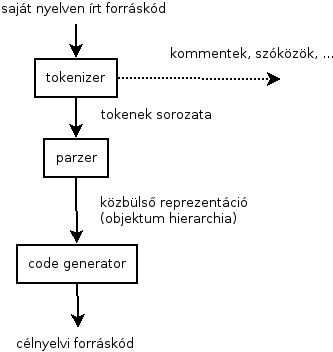
\includegraphics[scale=1]{kepek/process.png}
\caption{A keresztfordítás lépései}
\label{fig:process}
\end{figure}

\subsection{Tokenizálás}

Az tokenizálás a fordítás első lépése lesz, ebben a lépésben a felhasználó által megadott programkód beolvasásra kerül, majd a program szétbontja azt és megvizsgálja az egyes elemeket. A tokenizer minden elemhez hozzá kell tudjon rendelni a program egy tokent, így a tokenizer visszatérési értéke tokenek egy sorozata lesz.

A tokenek sorozatában nem szerepelnek a különböző fehér karakterek, mint a szóköz, újsor, tabulátor karakter, mivel a tokenizer a feldolgozás során ezeket az elemeket, mivel ezek csak az olvashatóságot növelik a kódban, a feldolgozásához, fordításhoz plusz információval nem járulnak hozzá, törli.

Ezután a többi tokent a megadott reguláris kifejezések alapján hozza létre. A leggyakoribb tokenek közül néhány példa:
szám literál: \texttt{[0-9\_]+}
szöveg literál: \texttt{[a-zA-Z0-9\_]+}
zárójelek: \texttt{(} és \texttt{)}
fehér karakterek:
\begin{verbatim}
(\\n | \\r | \\r\\n | \\f | \\t)+
\end{verbatim}

A tokenizer általában egy külön programrész, osztály a feldolgozóban, melyet általában lexernek is neveznek. Ezt az osztályt külön programok segítségével lehet megalkotni, melyeket lexer generatornak nevezik. Az interneten többféle ilyen generátor is található, melyeket segítségül hívva meg lehet alkotni a feldolgozó osztályt.

Fontos, hogy ezeknek a generátoroknak meg kell adni egy szintaktikai leírást, mely alapján a lexert létrehozzák, azonban figyelni kell arra, hogy az adott generátornak megfelelő módon, és a általunk megadott nyelvre illeszkedő kifejezéseket adjunk meg.

A fellelhető generátorok közül jelen esetben olyanok közül kell választani amelyek a reguláris kifejezések segítségével adják meg a feldolgozási elemeket. Ilyenek  például az AnnoFlex, JFlex programok, ezekről részletesebben a szintaktikai elemzés fejezetben esik szó.

A megvalósításkor nehézséget okozott a fentebb említett választás és szintaktikai leírás. Mivel a korábbi tanulmányaim során ilyenre nem került sor, a generátor általt felhasznált szintaktikai leírás megvalósítása néhány esetben hibára futott. Ami ebben segítséget jelentett, az az AnnoFlex programban megadott példa kód volt, mely alapján további reguláris kifejezéseket fel lehetett venni.

\subsection{Parser}

A tokenek sorozata ezután átkerül a feldolgozás következő lépéseként a parserhez. A parser osztályt, mely a kapott kódot feldolgozza, szintén előtte definiálni kell, melyet az adott nyelvhez kapcsolódó megadott szintaktika, illetve egy parser generator végezhet el.

A lexer generatorthoz hasonlóan a parser generator is megtalálható az interneten. Fontos megjegyezni, hogy olyan parser és lexer generatort érdemes választani, mely a lehető legjobban együtt tud műküdik. Ilyen például a JFlex és a CUP generátor, mely generátort úgy terveztek, hogy egymással együttműködve tudnak működik.

A CUP generátort emellett magában is használható egy adott token sorozat feldolgozására, ezekről részletesebben szintén a szintaktikai elemzés fejezetben esik szó.

Szintén nehézséget okozott a megfelelő parser generátor kiválasztása, hiszen annak olyannak kell lennie, hogy a kiválasztott lexer generátorral együtt tudjon működni, az az által generált eredményhalmazt be tudja olvasni. Itt is felmerültek a fájl szintaktikai megvalósításakor fellépő hibák. Sajnos a CUP parser generátor leírása nem volt annyira részletes ez ügyben, így a hibák javítása hosszabb időt vett igénybe.

\subsection{Kód generálás}

Az utolsó lépés, hogy miután a parser generator által létrehozott objektum hierarchia elkészült, ebből a program elvégzi a konvertálást, és gíy jön létre majd a célnyelvi forráskód, ami már az adott nyelv szintaktikájának megfelelő és felhasználható a programozó izlése szerint.
